\begin{frame}{Zugfolge f�r $n=3$ und $k=3$}
\only<1>{
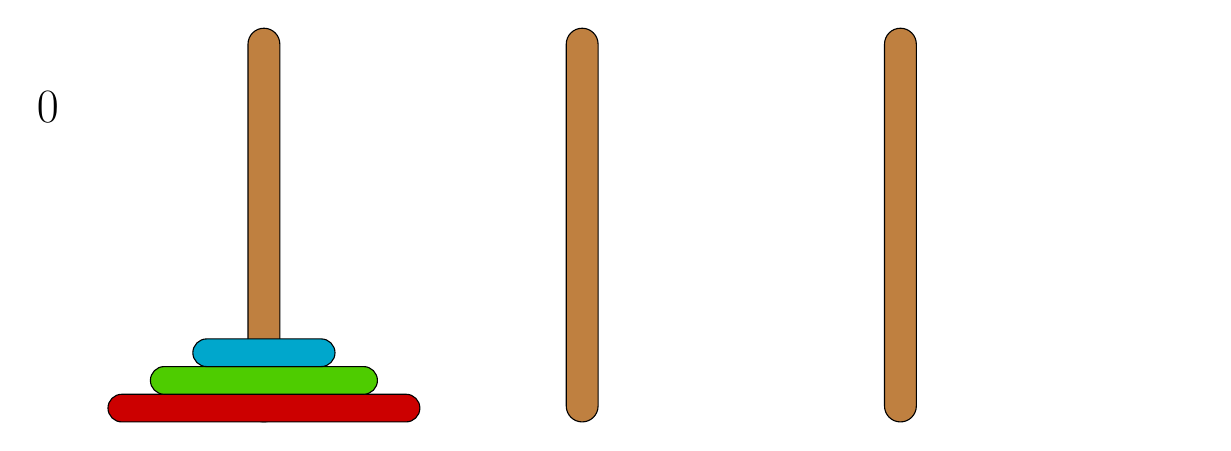
\begin{tikzpicture}
\pgfmathsetlengthmacro\diskheight{10};
\pgfmathsetmacro\k{3};
\pgfmathsetlengthmacro\step{\textwidth/\k};
\node[opacity = 1] at (1.5,4) {\LARGE 0};
\draw[color = white] (\step/2,0) -- (\textwidth+\step,0);
\foreach \n in {1,...,\k} \draw [fill = brown, draw = black, rounded corners = \step/20] (\step*\n,0) rectangle (\step*\n+\step/10,5);
\definecolor{mycolor}{rgb:hsb}{0.00,1,0.8}
\draw [fill = mycolor, draw = black, rounded corners = \diskheight/2] (\step*1+\step/20-\step*0.49,\diskheight*0) rectangle (\step*1+\step/20+\step*0.49,\diskheight*1);
\definecolor{mycolor}{rgb:hsb}{0.27,1,0.8}
\draw [fill = mycolor, draw = black, rounded corners = \diskheight/2] (\step*1+\step/20-\step*0.3566666666666667,\diskheight*1) rectangle (\step*1+\step/20+\step*0.3566666666666667,\diskheight*2);
\definecolor{mycolor}{rgb:hsb}{0.53,1,0.8}
\draw [fill = mycolor, draw = black, rounded corners = \diskheight/2] (\step*1+\step/20-\step*0.22333333333333333,\diskheight*2) rectangle (\step*1+\step/20+\step*0.22333333333333333,\diskheight*3);
\end{tikzpicture}
}
\only<2>{
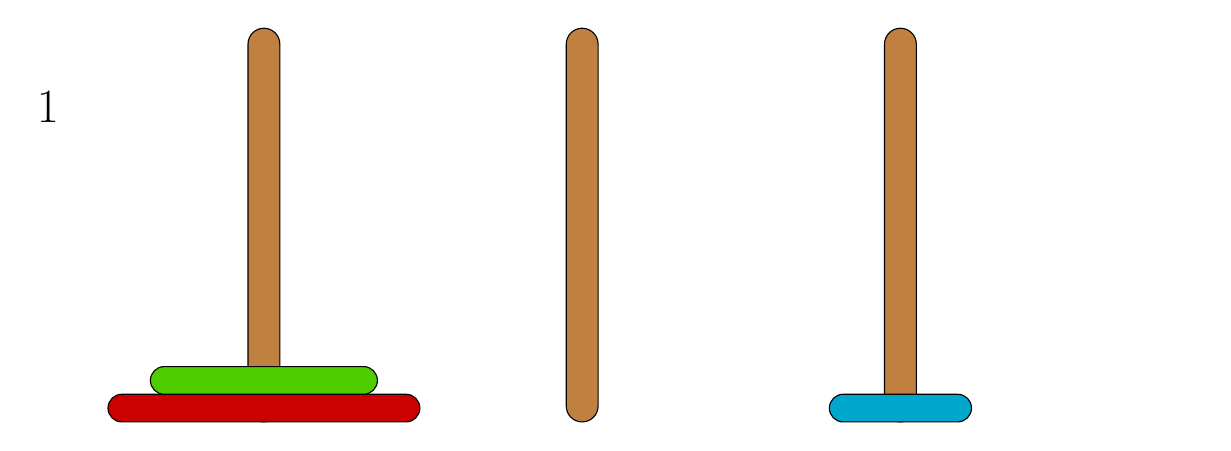
\begin{tikzpicture}
\pgfmathsetlengthmacro\diskheight{10};
\pgfmathsetmacro\k{3};
\pgfmathsetlengthmacro\step{\textwidth/\k};
\node[opacity = 1] at (1.5,4) {\LARGE 1};
\draw[color = white] (\step/2,0) -- (\textwidth+\step,0);
\foreach \n in {1,...,\k} \draw [fill = brown, draw = black, rounded corners = \step/20] (\step*\n,0) rectangle (\step*\n+\step/10,5);
\definecolor{mycolor}{rgb:hsb}{0.00,1,0.8}
\draw [fill = mycolor, draw = black, rounded corners = \diskheight/2] (\step*1+\step/20-\step*0.49,\diskheight*0) rectangle (\step*1+\step/20+\step*0.49,\diskheight*1);
\definecolor{mycolor}{rgb:hsb}{0.27,1,0.8}
\draw [fill = mycolor, draw = black, rounded corners = \diskheight/2] (\step*1+\step/20-\step*0.3566666666666667,\diskheight*1) rectangle (\step*1+\step/20+\step*0.3566666666666667,\diskheight*2);
\definecolor{mycolor}{rgb:hsb}{0.53,1,0.8}
\draw [fill = mycolor, draw = black, rounded corners = \diskheight/2] (\step*3+\step/20-\step*0.22333333333333333,\diskheight*0) rectangle (\step*3+\step/20+\step*0.22333333333333333,\diskheight*1);
\end{tikzpicture}
}
\only<3>{
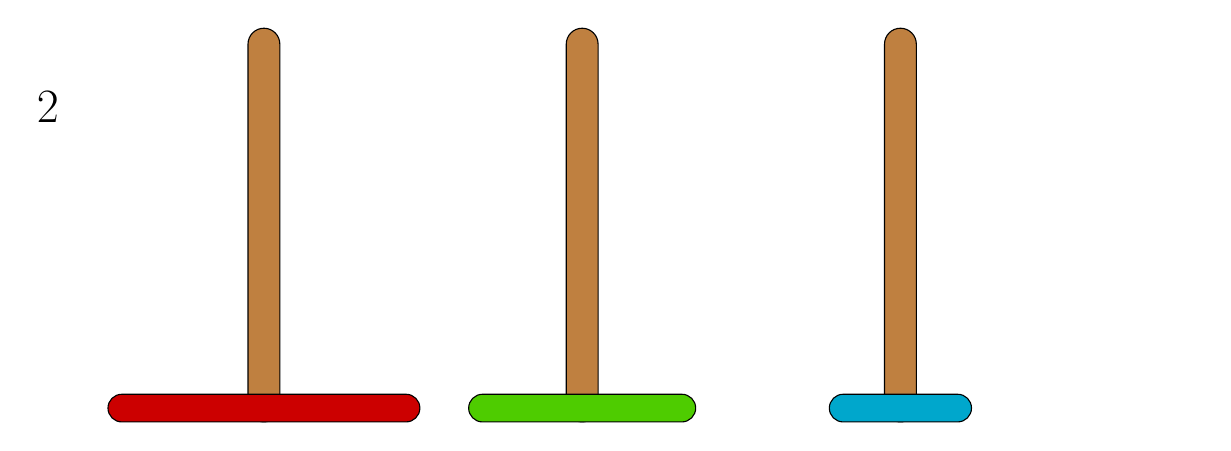
\begin{tikzpicture}
\pgfmathsetlengthmacro\diskheight{10};
\pgfmathsetmacro\k{3};
\pgfmathsetlengthmacro\step{\textwidth/\k};
\node[opacity = 1] at (1.5,4) {\LARGE 2};
\draw[color = white] (\step/2,0) -- (\textwidth+\step,0);
\foreach \n in {1,...,\k} \draw [fill = brown, draw = black, rounded corners = \step/20] (\step*\n,0) rectangle (\step*\n+\step/10,5);
\definecolor{mycolor}{rgb:hsb}{0.00,1,0.8}
\draw [fill = mycolor, draw = black, rounded corners = \diskheight/2] (\step*1+\step/20-\step*0.49,\diskheight*0) rectangle (\step*1+\step/20+\step*0.49,\diskheight*1);
\definecolor{mycolor}{rgb:hsb}{0.27,1,0.8}
\draw [fill = mycolor, draw = black, rounded corners = \diskheight/2] (\step*2+\step/20-\step*0.3566666666666667,\diskheight*0) rectangle (\step*2+\step/20+\step*0.3566666666666667,\diskheight*1);
\definecolor{mycolor}{rgb:hsb}{0.53,1,0.8}
\draw [fill = mycolor, draw = black, rounded corners = \diskheight/2] (\step*3+\step/20-\step*0.22333333333333333,\diskheight*0) rectangle (\step*3+\step/20+\step*0.22333333333333333,\diskheight*1);
\end{tikzpicture}
}
\only<4>{
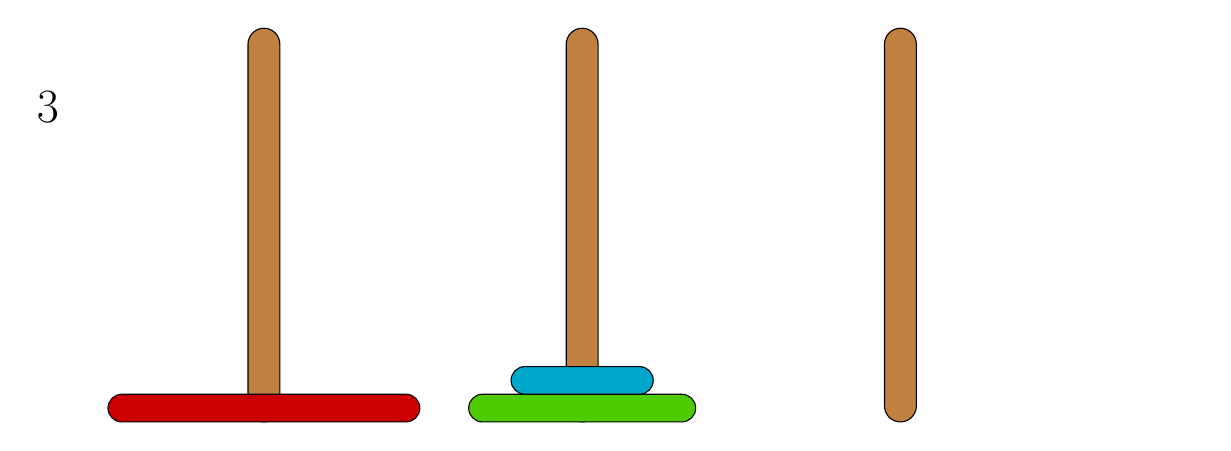
\begin{tikzpicture}
\pgfmathsetlengthmacro\diskheight{10};
\pgfmathsetmacro\k{3};
\pgfmathsetlengthmacro\step{\textwidth/\k};
\node[opacity = 1] at (1.5,4) {\LARGE 3};
\draw[color = white] (\step/2,0) -- (\textwidth+\step,0);
\foreach \n in {1,...,\k} \draw [fill = brown, draw = black, rounded corners = \step/20] (\step*\n,0) rectangle (\step*\n+\step/10,5);
\definecolor{mycolor}{rgb:hsb}{0.00,1,0.8}
\draw [fill = mycolor, draw = black, rounded corners = \diskheight/2] (\step*1+\step/20-\step*0.49,\diskheight*0) rectangle (\step*1+\step/20+\step*0.49,\diskheight*1);
\definecolor{mycolor}{rgb:hsb}{0.27,1,0.8}
\draw [fill = mycolor, draw = black, rounded corners = \diskheight/2] (\step*2+\step/20-\step*0.3566666666666667,\diskheight*0) rectangle (\step*2+\step/20+\step*0.3566666666666667,\diskheight*1);
\definecolor{mycolor}{rgb:hsb}{0.53,1,0.8}
\draw [fill = mycolor, draw = black, rounded corners = \diskheight/2] (\step*2+\step/20-\step*0.22333333333333333,\diskheight*1) rectangle (\step*2+\step/20+\step*0.22333333333333333,\diskheight*2);
\end{tikzpicture}
}
\only<5>{
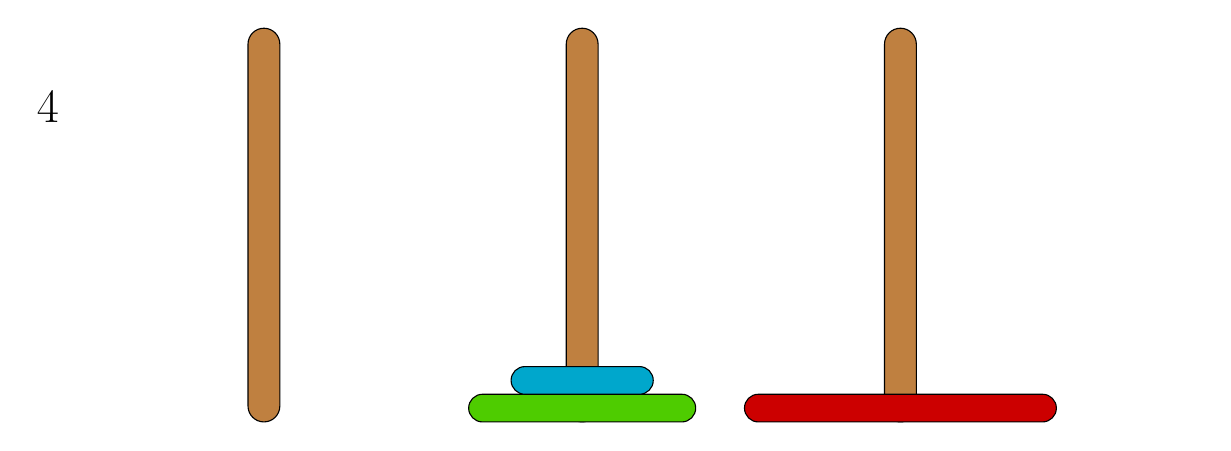
\begin{tikzpicture}
\pgfmathsetlengthmacro\diskheight{10};
\pgfmathsetmacro\k{3};
\pgfmathsetlengthmacro\step{\textwidth/\k};
\node[opacity = 1] at (1.5,4) {\LARGE 4};
\draw[color = white] (\step/2,0) -- (\textwidth+\step,0);
\foreach \n in {1,...,\k} \draw [fill = brown, draw = black, rounded corners = \step/20] (\step*\n,0) rectangle (\step*\n+\step/10,5);
\definecolor{mycolor}{rgb:hsb}{0.27,1,0.8}
\draw [fill = mycolor, draw = black, rounded corners = \diskheight/2] (\step*2+\step/20-\step*0.3566666666666667,\diskheight*0) rectangle (\step*2+\step/20+\step*0.3566666666666667,\diskheight*1);
\definecolor{mycolor}{rgb:hsb}{0.53,1,0.8}
\draw [fill = mycolor, draw = black, rounded corners = \diskheight/2] (\step*2+\step/20-\step*0.22333333333333333,\diskheight*1) rectangle (\step*2+\step/20+\step*0.22333333333333333,\diskheight*2);
\definecolor{mycolor}{rgb:hsb}{0.00,1,0.8}
\draw [fill = mycolor, draw = black, rounded corners = \diskheight/2] (\step*3+\step/20-\step*0.49,\diskheight*0) rectangle (\step*3+\step/20+\step*0.49,\diskheight*1);
\end{tikzpicture}
}
\only<6>{
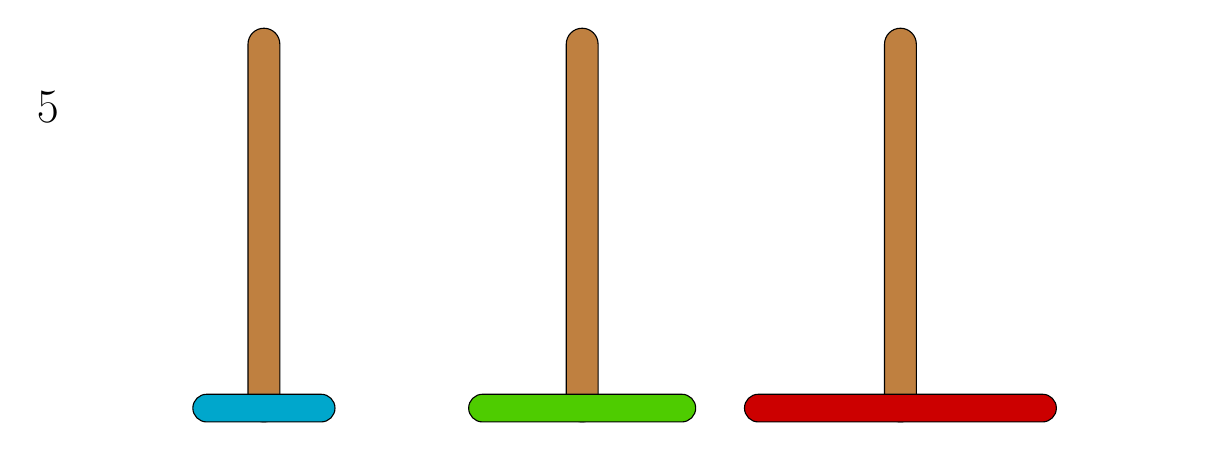
\begin{tikzpicture}
\pgfmathsetlengthmacro\diskheight{10};
\pgfmathsetmacro\k{3};
\pgfmathsetlengthmacro\step{\textwidth/\k};
\node[opacity = 1] at (1.5,4) {\LARGE 5};
\draw[color = white] (\step/2,0) -- (\textwidth+\step,0);
\foreach \n in {1,...,\k} \draw [fill = brown, draw = black, rounded corners = \step/20] (\step*\n,0) rectangle (\step*\n+\step/10,5);
\definecolor{mycolor}{rgb:hsb}{0.53,1,0.8}
\draw [fill = mycolor, draw = black, rounded corners = \diskheight/2] (\step*1+\step/20-\step*0.22333333333333333,\diskheight*0) rectangle (\step*1+\step/20+\step*0.22333333333333333,\diskheight*1);
\definecolor{mycolor}{rgb:hsb}{0.27,1,0.8}
\draw [fill = mycolor, draw = black, rounded corners = \diskheight/2] (\step*2+\step/20-\step*0.3566666666666667,\diskheight*0) rectangle (\step*2+\step/20+\step*0.3566666666666667,\diskheight*1);
\definecolor{mycolor}{rgb:hsb}{0.00,1,0.8}
\draw [fill = mycolor, draw = black, rounded corners = \diskheight/2] (\step*3+\step/20-\step*0.49,\diskheight*0) rectangle (\step*3+\step/20+\step*0.49,\diskheight*1);
\end{tikzpicture}
}
\only<7>{
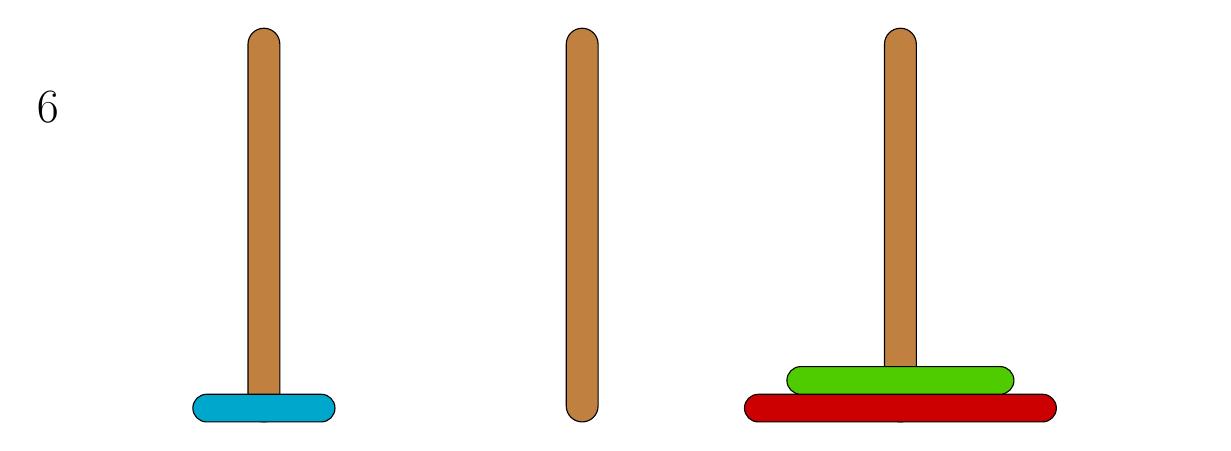
\begin{tikzpicture}
\pgfmathsetlengthmacro\diskheight{10};
\pgfmathsetmacro\k{3};
\pgfmathsetlengthmacro\step{\textwidth/\k};
\node[opacity = 1] at (1.5,4) {\LARGE 6};
\draw[color = white] (\step/2,0) -- (\textwidth+\step,0);
\foreach \n in {1,...,\k} \draw [fill = brown, draw = black, rounded corners = \step/20] (\step*\n,0) rectangle (\step*\n+\step/10,5);
\definecolor{mycolor}{rgb:hsb}{0.53,1,0.8}
\draw [fill = mycolor, draw = black, rounded corners = \diskheight/2] (\step*1+\step/20-\step*0.22333333333333333,\diskheight*0) rectangle (\step*1+\step/20+\step*0.22333333333333333,\diskheight*1);
\definecolor{mycolor}{rgb:hsb}{0.00,1,0.8}
\draw [fill = mycolor, draw = black, rounded corners = \diskheight/2] (\step*3+\step/20-\step*0.49,\diskheight*0) rectangle (\step*3+\step/20+\step*0.49,\diskheight*1);
\definecolor{mycolor}{rgb:hsb}{0.27,1,0.8}
\draw [fill = mycolor, draw = black, rounded corners = \diskheight/2] (\step*3+\step/20-\step*0.3566666666666667,\diskheight*1) rectangle (\step*3+\step/20+\step*0.3566666666666667,\diskheight*2);
\end{tikzpicture}
}
\only<8>{
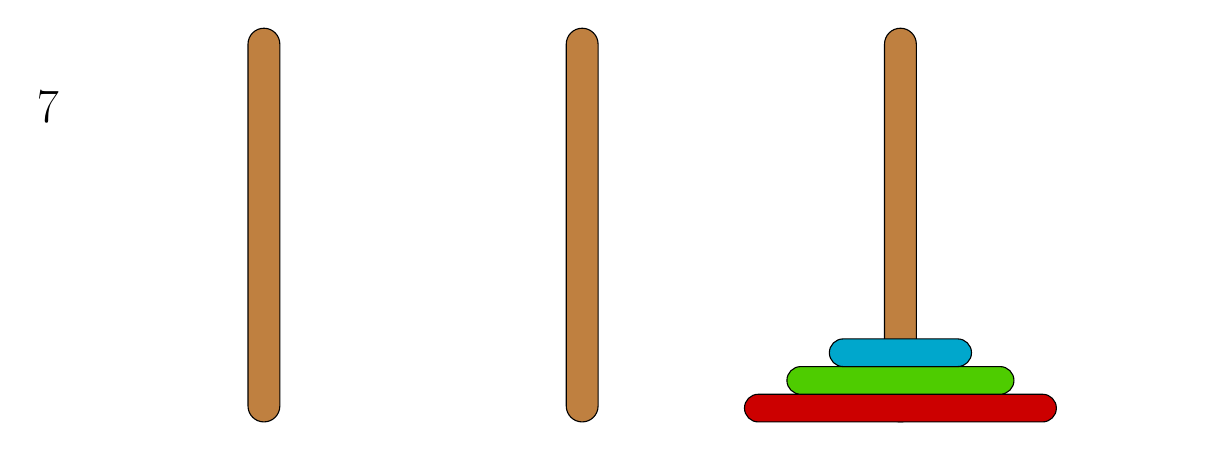
\begin{tikzpicture}
\pgfmathsetlengthmacro\diskheight{10};
\pgfmathsetmacro\k{3};
\pgfmathsetlengthmacro\step{\textwidth/\k};
\node[opacity = 1] at (1.5,4) {\LARGE 7};
\draw[color = white] (\step/2,0) -- (\textwidth+\step,0);
\foreach \n in {1,...,\k} \draw [fill = brown, draw = black, rounded corners = \step/20] (\step*\n,0) rectangle (\step*\n+\step/10,5);
\definecolor{mycolor}{rgb:hsb}{0.00,1,0.8}
\draw [fill = mycolor, draw = black, rounded corners = \diskheight/2] (\step*3+\step/20-\step*0.49,\diskheight*0) rectangle (\step*3+\step/20+\step*0.49,\diskheight*1);
\definecolor{mycolor}{rgb:hsb}{0.27,1,0.8}
\draw [fill = mycolor, draw = black, rounded corners = \diskheight/2] (\step*3+\step/20-\step*0.3566666666666667,\diskheight*1) rectangle (\step*3+\step/20+\step*0.3566666666666667,\diskheight*2);
\definecolor{mycolor}{rgb:hsb}{0.53,1,0.8}
\draw [fill = mycolor, draw = black, rounded corners = \diskheight/2] (\step*3+\step/20-\step*0.22333333333333333,\diskheight*2) rectangle (\step*3+\step/20+\step*0.22333333333333333,\diskheight*3);
\end{tikzpicture}
}
\end{frame}